\chapter{Järjestäminen}

\index{järjestäminen}

\emph{Järjestäminen} on keskeinen algoritmiikan ongelma,
jossa tehtävänä on jär\-jestää $n$ alkiota sisältävä
taulukko suuruusjärjestykseen.
Esimerkiksi jos meil\-lä on taulukko $[5,2,4,2,6,1]$ ja
järjestämme sen alkiot pienimmästä suurimpaan,
tuloksena on taulukko $[1,2,2,4,5,6]$.

Tavoitteemme on toteuttaa järjestäminen
\emph{tehokkaasti}.
On helppoa järjes\-tää taulukko ajassa $O(n^2)$,
mutta tämä on liian hidasta suurella taulukolla.
Tässä luvussa opimme kaksi tehokasta
järjestämisalgoritmia, jotka vievät aikaa vain $O(n \log n)$.
Toisaalta osoittautuu, että ei ole olemassa
yleistä järjestämisalgoritmia, joka toimisi nopeammin
kuin $O(n \log n)$.

Voimme käyttää järjestämistä monella tavalla
algoritmien suunnittelussa.
Usein voimme helpottaa ongelman ratkaisemista
järjestämällä ensin aineiston.
Esimerkiksi jos haluamme tutkia,
mikä alkio esiintyy useimmiten taulukossa,
voimme järjestää ensin taulukon,
jolloin yhtä suuret alkiot päätyvät vierekkäin.
Tämän jälkeen meidän riittää käydä taulukko läpi
ja etsiä siitä pisin samaa alkiota toistava osuus.

\section{Järjestäminen ajassa $O(n^2)$}

\index{lisäysjärjestäminen}

Tutustumme aluksi yksinkertaiseen järjestämisalgoritmiin,
joka järjestää $n$-alkioisen taulukon ajassa $O(n^2)$ kahden silmukan avulla.
Vaikka algoritmi ei ole nopea, se on tutustumisen arvoinen
ja antaa hyvän lähtökohdan tehokkaampien algoritmien
suunnittelemiselle.

\subsection{Lisäysjärjestäminen}

\emph{Lisäysjärjestäminen} käy läpi taulukon
vasemmalta oikealle.
Kun algoritmi tulee tiettyyn taulukon kohtaan,
se siirtää kyseisessä kohdassa olevan alkion
oikeaan paikkaan taulukon
alkuosassa niin, että taulukon alkuosa
on tämän jälkeen järjestyksessä.
Niinpä kun algoritmi pääsee taulukon loppuun,
koko taulukko on järjestyksessä.

\begin{figure}
\center
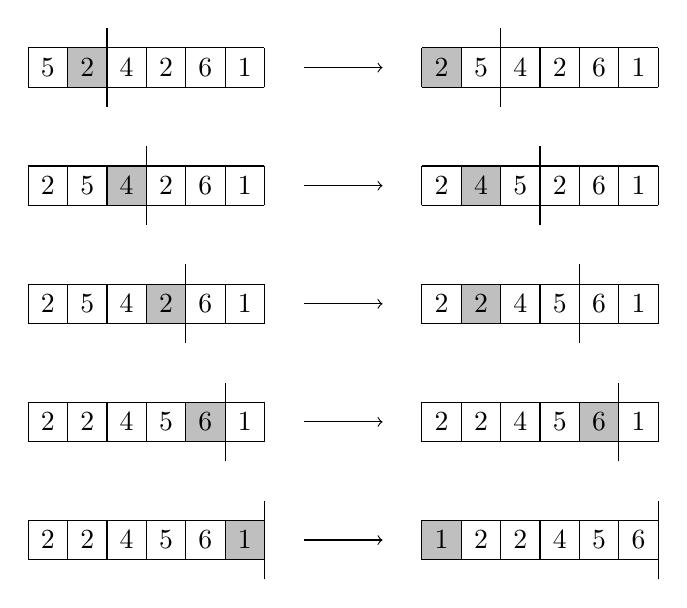
\begin{tikzpicture}[scale=0.5]
\begin{scope}
\fill[lightgray] (1,0) rectangle (2,1);
\draw (0,0) grid (6,1);
\foreach \x/\v in {0/5,1/2,2/4,3/2,4/6,5/1} \node at (0.5+\x,0.5) {\v};
\draw (2,-0.5) -- (2,1.5);
\draw[->] (7,0.5) -- (9,0.5);
\end{scope}
\begin{scope}[xshift=10cm]
\fill[lightgray] (0,0) rectangle (1,1);
\draw (0,0) grid (6,1);
\foreach \x/\v in {0/2,1/5,2/4,3/2,4/6,5/1} \node at (0.5+\x,0.5) {\v};
\draw (2,-0.5) -- (2,1.5);
\end{scope}
\begin{scope}[yshift=-3cm]
\fill[lightgray] (2,0) rectangle (3,1);
\draw (0,0) grid (6,1);
\foreach \x/\v in {0/2,1/5,2/4,3/2,4/6,5/1} \node at (0.5+\x,0.5) {\v};
\draw (3,-0.5) -- (3,1.5);
\draw[->] (7,0.5) -- (9,0.5);
\end{scope}
\begin{scope}[yshift=-3cm,xshift=10cm]
\fill[lightgray] (1,0) rectangle (2,1);
\draw (0,0) grid (6,1);
\foreach \x/\v in {0/2,1/4,2/5,3/2,4/6,5/1} \node at (0.5+\x,0.5) {\v};
\draw (3,-0.5) -- (3,1.5);
\end{scope}
\begin{scope}[yshift=-6cm]
\fill[lightgray] (3,0) rectangle (4,1);
\draw (0,0) grid (6,1);
\foreach \x/\v in {0/2,1/5,2/4,3/2,4/6,5/1} \node at (0.5+\x,0.5) {\v};
\draw (4,-0.5) -- (4,1.5);
\draw[->] (7,0.5) -- (9,0.5);
\end{scope}
\begin{scope}[yshift=-6cm,xshift=10cm]
\fill[lightgray] (1,0) rectangle (2,1);
\draw (0,0) grid (6,1);
\foreach \x/\v in {0/2,1/2,2/4,3/5,4/6,5/1} \node at (0.5+\x,0.5) {\v};
\draw (4,-0.5) -- (4,1.5);
\end{scope}
\begin{scope}[yshift=-9cm]
\fill[lightgray] (4,0) rectangle (5,1);
\draw (0,0) grid (6,1);
\foreach \x/\v in {0/2,1/2,2/4,3/5,4/6,5/1} \node at (0.5+\x,0.5) {\v};
\draw (5,-0.5) -- (5,1.5);
\draw[->] (7,0.5) -- (9,0.5);
\end{scope}
\begin{scope}[yshift=-9cm,xshift=10cm]
\fill[lightgray] (4,0) rectangle (5,1);
\draw (0,0) grid (6,1);
\foreach \x/\v in {0/2,1/2,2/4,3/5,4/6,5/1} \node at (0.5+\x,0.5) {\v};
\draw (5,-0.5) -- (5,1.5);
\end{scope}
\begin{scope}[yshift=-12cm]
\fill[lightgray] (5,0) rectangle (6,1);
\draw (0,0) grid (6,1);
\foreach \x/\v in {0/2,1/2,2/4,3/5,4/6,5/1} \node at (0.5+\x,0.5) {\v};
\draw (6,-0.5) -- (6,1.5);
\draw[->] (7,0.5) -- (9,0.5);
\end{scope}
\begin{scope}[yshift=-12cm,xshift=10cm]
\fill[lightgray] (0,0) rectangle (1,1);
\draw (0,0) grid (6,1);
\foreach \x/\v in {0/1,1/2,2/2,3/4,4/5,5/6} \node at (0.5+\x,0.5) {\v};
\draw (6,-0.5) -- (6,1.5);
\end{scope}
\end{tikzpicture}
\caption{Lisäysjärjestäminen taulukolle $[5,2,4,2,6,1]$.}
\label{fig:lisjar}
\end{figure}

Kuva \ref{fig:lisjar} näyttää esimerkin lisäysjärjestämisen
toiminnasta, kun järjes\-tämme taulukon $[5,2,4,2,6,1]$.
Jokaisella rivillä siirrämme harmaataustaisen alkion
sen oikealle paikalle taulukon alkuosassa.
Pystyviiva ilmaisee kohdan, johon asti taulukko on järjestyksessä
siirron jälkeen.
Lopulta saamme aikaan järjestetyn taulukon $[1,2,2,4,5,6]$.

Seuraava koodi toteuttaa lisäysjärjestämisen:

\begin{code}
for i = 1 to n-1
    j = i-1
    while j >= 0 and taulu[j] > taulu[j+1]
        swap(taulu[j],taulu[j+1])
        j--
\end{code}

Koodissa komento \texttt{swap} vaihtaa keskenään
sille annetut alkiot.
Jokaisen indeksin $i$ kohdalla siirrämme taulukon
kohdassa $i$ olevan alkion sen oikealle paikalle
taulukon alkuosassa.
Teemme tämän vaihtamalla joka askeleella keskenään
alkion ja sen vasemmalla puolella olevan alkion
niin kauan, kunnes alkio on oikealla paikalla.

Lisäysjärjestämisen tehokkuus riippuu siitä,
mikä on järjestettävän taulukon sisältö.
Algoritmi toimii sitä paremmin, mitä lähempänä järjestystä
taulukko on valmiiksi.
Jos taulukko on järjestyksessä,
aikaa kuluu vain $O(n)$, koska meidän ei tarvitse siirtää
mitään alkioita.
Pahin tapaus algoritmille on kuitenkin, että taulukko on
\emph{käänteisessä} järjestyksessä,
jolloin joudumme siirtämään jokaisen alkion
taulukon alkuun ja aikaa kuluu $O(n^2)$.

\subsection{Inversiot}

\index{inversio}

Hyödyllinen käsite järjestämisalgoritmien analysoinnissa
on \emph{inversio}: kaksi taulukossa olevaa alkiota,
jotka ovat väärässä järjestyksessä.
Esimerkiksi taulukossa $[3,1,4,2]$ on kolme inversiota:
$(3,1)$, $(3,2)$ ja $(4,2)$.
Inversioiden määrä kertoo meille taulukon järjestyksestä:
mitä vähemmän inversioita taulukossa on,
sitä lähempänä se on järjestystä.
Erityisesti taulukko on järjestyksessä tarkalleen silloin,
kun siinä ei ole yhtään inversiota.

Kun järjestämisalgoritmi järjestää taulukon,
se \emph{poistaa} siitä inversioita.
Lisäysjärjestämisen tapauksessa aina kun
algoritmi vaihtaa kaksi alkiota keskenään,
se poistaa taulukosta yhden inversion.
Niinpä lisäysjärjestämisen työmäärä on yhtä suuri
kuin järjestettävän taulukon inversioiden määrä.

Olemme jo todenneet, että pahin mahdollinen syöte
lisäysjärjestämiselle on käänteisessä järjestyksessä oleva taulukko.
Tällaisessa taulukossa jokainen alkiopari muodostaa inversion,
joten inversioiden määrä on
\[\frac{n(n-1)}{2}=O(n^2).\]
Entä kuinka hyvin algoritmi toimii \emph{keskimäärin}?
Jos oletamme, että taulukossa on $n$ eri alkiota satunnaisessa
järjestyksessä, alkiopari muodostaa inversion todennäköisyydellä $1/2$.
Niinpä inversioiden määrän \emph{odotusarvo} on
\[\frac{n(n-1)}{4}=O(n^2),\]
eli aikaa kuluu neliöllinen määrä myös keskimääräisessä
tapauksessa.

Syy lisäysjärjestämisen hitauteen on siis,
että se ei poista taulukosta inversioita riittävän tehokkaasti.
Jos haluamme kehittää paremman järjestämis\-algoritmin,
meidän täytyy suunnitella se niin, että se voi poistaa
useita inversioita \emph{yhtä aikaa}.
Käytännössä algoritmin täytyy pystyä siirtämään
väärässä paikassa oleva alkio tehokkaasti taulukon
toiselle puolelle.

\section{Järjestäminen ajassa $O(n \log n)$}

Seuraavaksi tutustumme kahteen tehokkaaseen
järjestämisalgoritmiin, jotka perustuvat rekursioon.
Molemmissa algoritmeissa on ideana,
että kun haluamme järjestää taulukon,
jaamme sen kahteen pienempään osaan
ja järjestämme ne rekursiivisesti.
Tämän jälkeen yhdistämme järjestetyt osataulukot
kokonaiseksi järjestetyksi taulukoksi.

\subsection{Lomitusjärjestäminen}

\index{lomitusjärjestäminen}

\begin{figure}
\center
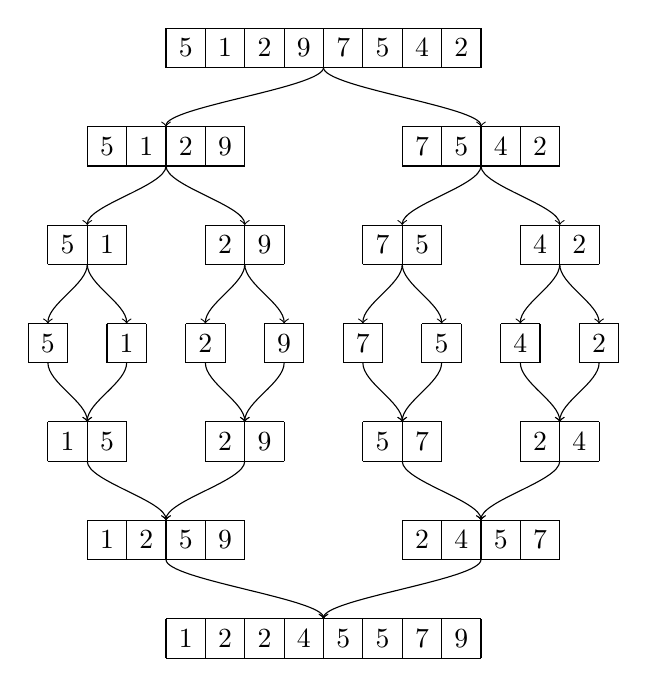
\begin{tikzpicture}[scale=0.5]
\begin{scope}
\draw (0,0) grid (8,1);
\foreach \x/\v in {0/5,1/1,2/2,3/9,4/7,5/5,6/4,7/2} \node at (0.5+\x,0.5) {\v};
\draw[->] (4,0) .. controls (4,-0.5) and (0,-1) .. (0,-1.5);
\draw[->] (4,0) .. controls (4,-0.5) and (8,-1) .. (8,-1.5);
\end{scope}
\begin{scope}[yshift=-2.5cm,xshift=-2cm]
\draw (0,0) grid (4,1);
\draw (8,0) grid (12,1);
\foreach \x/\v in {0/5,1/1,2/2,3/9,8/7,9/5,10/4,11/2} \node at (0.5+\x,0.5) {\v};
\draw[->] (2,0) .. controls (2,-0.5) and (0,-1) .. (0,-1.5);
\draw[->] (2,0) .. controls (2,-0.5) and (4,-1) .. (4,-1.5);
\draw[->] (10,0) .. controls (10,-0.5) and (8,-1) .. (8,-1.5);
\draw[->] (10,0) .. controls (10,-0.5) and (12,-1) .. (12,-1.5);
\end{scope}
\begin{scope}[yshift=-5cm,xshift=-3cm]
\draw (0,0) grid (2,1);
\draw (4,0) grid (6,1);
\draw (8,0) grid (10,1);
\draw (12,0) grid (14,1);
\foreach \x/\v in {0/5,1/1,4/2,5/9,8/7,9/5,12/4,13/2} \node at (0.5+\x,0.5) {\v};
\draw[->] (1,0) .. controls (1,-0.5) and (0,-1) .. (0,-1.5);
\draw[->] (1,0) .. controls (1,-0.5) and (2,-1) .. (2,-1.5);
\draw[->] (5,0) .. controls (5,-0.5) and (4,-1) .. (4,-1.5);
\draw[->] (5,0) .. controls (5,-0.5) and (6,-1) .. (6,-1.5);
\draw[->] (9,0) .. controls (9,-0.5) and (8,-1) .. (8,-1.5);
\draw[->] (9,0) .. controls (9,-0.5) and (10,-1) .. (10,-1.5);
\draw[->] (13,0) .. controls (13,-0.5) and (12,-1) .. (12,-1.5);
\draw[->] (13,0) .. controls (13,-0.5) and (14,-1) .. (14,-1.5);
\end{scope}
\begin{scope}[yshift=-7.5cm,xshift=-3.5cm]
\draw (0,0) grid (1,1);
\draw (2,0) grid (3,1);
\draw (4,0) grid (5,1);
\draw (6,0) grid (7,1);
\draw (8,0) grid (9,1);
\draw (10,0) grid (11,1);
\draw (12,0) grid (13,1);
\draw (14,0) grid (15,1);
\foreach \x/\v in {0/5,2/1,4/2,6/9,8/7,10/5,12/4,14/2} \node at (0.5+\x,0.5) {\v};
\draw[->] (0.5,0) .. controls (0.5,-0.5) and (1.5,-1) .. (1.5,-1.5);
\draw[->] (2.5,0) .. controls (2.5,-0.5) and (1.5,-1) .. (1.5,-1.5);
\draw[->] (4.5,0) .. controls (4.5,-0.5) and (5.5,-1) .. (5.5,-1.5);
\draw[->] (6.5,0) .. controls (6.5,-0.5) and (5.5,-1) .. (5.5,-1.5);
\draw[->] (8.5,0) .. controls (8.5,-0.5) and (9.5,-1) .. (9.5,-1.5);
\draw[->] (10.5,0) .. controls (10.5,-0.5) and (9.5,-1) .. (9.5,-1.5);
\draw[->] (12.5,0) .. controls (12.5,-0.5) and (13.5,-1) .. (13.5,-1.5);
\draw[->] (14.5,0) .. controls (14.5,-0.5) and (13.5,-1) .. (13.5,-1.5);
\end{scope}
\begin{scope}[yshift=-10cm,xshift=-3cm]
\draw (0,0) grid (2,1);
\draw (4,0) grid (6,1);
\draw (8,0) grid (10,1);
\draw (12,0) grid (14,1);
\foreach \x/\v in {0/1,1/5,4/2,5/9,8/5,9/7,12/2,13/4} \node at (0.5+\x,0.5) {\v};
\draw[->] (1,0) .. controls (1,-0.5) and (3,-1) .. (3,-1.5);
\draw[->] (5,0) .. controls (5,-0.5) and (3,-1) .. (3,-1.5);
\draw[->] (9,0) .. controls (9,-0.5) and (11,-1) .. (11,-1.5);
\draw[->] (13,0) .. controls (13,-0.5) and (11,-1) .. (11,-1.5);
\end{scope}
\begin{scope}[yshift=-12.5cm,xshift=-2cm]
\draw (0,0) grid (4,1);
\draw (8,0) grid (12,1);
\foreach \x/\v in {0/1,1/2,2/5,3/9,8/2,9/4,10/5,11/7} \node at (0.5+\x,0.5) {\v};
\draw[->] (2,0) .. controls (2,-0.5) and (6,-1) .. (6,-1.5);
\draw[->] (10,0) .. controls (10,-0.5) and (6,-1) .. (6,-1.5);
\end{scope}
\begin{scope}[yshift=-15cm]
\draw (0,0) grid (8,1);
\foreach \x/\v in {0/1,1/2,2/2,3/4,4/5,5/5,6/7,7/9} \node at (0.5+\x,0.5) {\v};
\end{scope}
\end{tikzpicture}
\caption{Lomitusjärjestäminen taulukolle $[5,1,2,9,7,5,4,2]$.}
\label{fig:lomjar}
\end{figure}

\emph{Lomitusjärjestäminen} on rekursiivinen järjestämisalgoritmi,
joka perustuu taulukon puolituksiin.
Kun saamme järjestettäväksi $n$-kokoisen taulukon,
jaamme sen keskeltä kahdeksi osataulukoksi,
joissa molemmissa on noin $n/2$ alkiota.
Tämän jälkeen järjestämme osataulukot erikseen rekursiivisesti
ja \emph{lomitamme} sitten järjestetyt osataulukot niin,
että niistä muodostuu kokonainen järjestetty taulukko.
Rekursio päättyy tapaukseen $n=1$, jolloin
taulukko on valmiiksi järjestyksessä eikä
tarvitse tehdä mitään.

Seuraava koodi esittää tarkemmin lomitusjärjestämisen toiminnan:

\begin{code}
function jarjesta(a,b)
    if a == b
        return
    k = (a+b)/2
    jarjesta(a,k-1)
    jarjesta(k,b)
    lomita(a,k-1,k,b)
\end{code}

Funktio \texttt{jarjesta} järjestää taulukon
välin $a \dots b$ (osataulukon kohdasta
$a$ kohtaan $b$), eli kun haluamme järjestää koko taulukon,
kutsumme funktiota parametreilla $a=0$ ja $b=n-1$.
Tarkastamme ensin, onko osataulukossa vain yksi alkio,
ja jos on, poistumme funktiosta.
Sitten laskemme muuttujaan $k$ järjestettävän välin keskikohdan
ja järjestämme vasemman ja oikean puoliskon rekursiivisesti.
Lopuksi kutsumme funktiota \texttt{lomita},
joka yhdistää järjestetyt puoliskot:

\begin{code}
function lomita(a1, b1, a2, b2)
    a = a1, b = b2
    for i = a to b
        if a2 > b2 or (a1 <= b1 and taulu[a1] < taulu[a2])
            apu[i] = taulu[a1]
            a1++
        else
            apu[i] = taulu[b1]
            b1++
    for i = a to b
        taulu[i] = apu[i]
\end{code}

Funktiolle annetaan välit $a_1 \dots b_1$ ja $a_2 \dots b_2$,
missä $b_1+1=a_2$.
Funktio olettaa, että näillä väleillä olevat 
taulukon alkiot on järjestetty,
ja se lomittaa alkiot niin, että funktion suorituksen jälkeen
taulukon koko väli $a_1 \dots b_2$ on järjestetty.
Funktion perustana on silmukka, joka käy läpi välejä
$a_1 \dots b_1$ ja $a_2 \dots b_2$ rinnakkain ja valitsee
aina seuraavaksi pienimmän alkion lopulliseen järjestykseen.
Jotta lomitus ei sotke taulukkoa,
funktio käyttää globaalia aputaulukkoa,
johon se ensin muodostaa järjestetyn osataulukon,
ja kopioi sitten alkiot aputaulukosta varsinaiseen taulukkoon.

Kuva \ref{fig:lomjar} näyttää, miten lomitusjärjestäminen
toimii, kun sille annetaan taulukko $[5,1,2,9,7,5,4,2]$.
Algoritmi puolittaa ensin taulukon kahdeksi osataulukoksi
$[5,1,2,9]$ ja $[7,5,4,2]$ ja järjestää molemmat
osataulukot kutsumalla itseään.
Kun algoritmi saa sitten järjestettäväksi taulukon $[5,1,2,9]$,
se jakaantuu jälleen osataulukoiksi $[5,1]$ ja $[2,9]$, jne.
Lopulta jäljellä on vain yhden alkion kokoisia
osataulukoita, jotka ovat valmiiksi järjestyksessä.
Tällöin rekursiivinen jakautuminen päättyy ja algoritmi
alkaa koota järjestettyjä osataulukkoja pienimmästä suurimpaan.

Nyt voimme määrittää, kuinka tehokas lomitusjärjestäminen on.
Koska jokainen funktion \texttt{jarjesta} kutsu
puolittaa taulukon koon, rekursiosta muodostuu
$O(\log n)$ tasoa  (kuva \ref{fig:lomjar}).
Ylimmällä tasolla on taulukko,
jossa on $n$ alkiota,
seuraavalla tasolla on kaksi taulukkoa,
joissa on $n/2$ alkiota,
seuraavalla tasolla on neljä taulukkoa,
joissa on $n/4$ alkiota, jne.
Funktio \texttt{lomita} toimii lineaarisessa ajassa,
joten kullakin tasolla taulukoiden lomittamiset vievät yhteensä
aikaa $O(n)$.
Niinpä algoritmin kokonaisaikavaativuus on $O(n \log n)$.

\subsection{Pikajärjestäminen}

\index{pikajärjestäminen}

\emph{Pikajärjestäminen} tarjoaa toisenlaisen rekursiivisen
lähestymistavan taulukon järjestämiseen.
Kun saamme järjestettäväksi taulukon, valitsemme ensin jonkin
sen alkioista \emph{jakoalkioksi}.
Tämän jälkeen siirrämme alkioita niin,
että jakoalkiota pienemmät alkiot ovat sen vasemmalla puolella,
suuremmat alkiot ovat sen oikealla puolella ja
yhtä suuret alkiot voivat olla kummalla tahansa puolella.
Lopuksi järjestämme rekursiivisesti osataulukot,
jotka muodostuvat jakoalkion vasemmalle ja oikealle puolelle.

Seuraava koodi esittää pikajärjestämisen toiminnan:

\begin{code}
function jarjesta(a, b)
    if a >= b
        return
    k = jako(a,b)
    jarjesta(a,k-1)
    jarjesta(k+1,b)
\end{code}

Funktio \texttt{jarjesta} järjestää taulukon välillä
$a \dots b$ olevat alkiot.
Jos väli on tyhjä tai siinä on vain yksi alkio,
funktio ei tee mitään.
Muuten funktio kutsuu funktiota \texttt{jako}, joka valitsee jakoalkion,
siirtää taulukon alkioita sen mukaisesti
ja palauttaa sitten kohdan $k$,
jossa jakoalkio on siirtojen jälkeen.
Tämän jälkeen taulukon vasen osa (väli $a \dots k-1$)
ja oikea osa (väli $k+1 \dots b$) järjestetään rekursiivisesti.

Funktion \texttt{jako} voi toteuttaa monella tavalla,
koska voimme valita minkä tahansa alkion jakoalkioksi ja
lisäksi on monia tapoja siirtää alkioita.
Käy\-tämme tässä esimerkkinä seuraavaa toteutusta:

\begin{code}
function jako(a,b):
    k = a
    for i = a+1 to b
        if taulu[i] < taulu[a]
            k += 1
            swap(taulu[i],taulu[k])
    swap(taulu[a],taulu[k])
    return k
\end{code}

Tässä jakoalkio on aina välin ensimmäinen alkio,
joka on kohdassa $a$.
Funktio käy läpi välin alkiot ja siirtää
jakoalkiota pienempiä alkioita taulukon alkuosaan.
Muuttuja $k$ määrittää kohdan,
johon seuraava pienempi alkio siirretään.
Lopuksi jakoalkio itse siirretään keskelle
kohtaan $k$, jonka funktio myös palauttaa.

\begin{figure}
\center
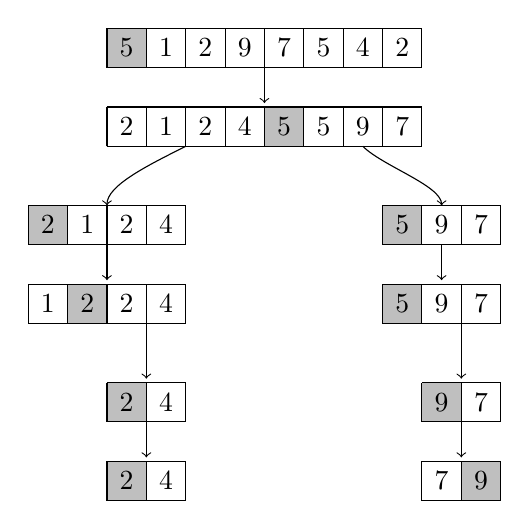
\begin{tikzpicture}[scale=0.5]
\begin{scope}
\fill[lightgray] (0,0) rectangle (1,1);
\draw (0,0) grid (8,1);
\foreach \x/\v in {0/5,1/1,2/2,3/9,4/7,5/5,6/4,7/2} \node at (0.5+\x,0.5) {\v};
\fill[lightgray] (4,-2) rectangle (5,-1);
\draw (0,-2) grid (8,-1);
\foreach \x/\v in {0/2,1/1,2/2,3/4,4/5,5/5,6/9,7/7} \node at (0.5+\x,-1.5) {\v};
\draw[->] (4,0) -- (4,-0.9);
\draw[->] (2,-2) .. controls (1,-2.5) and (0,-3) .. (0,-3.5);
\draw[->] (6.5,-2) .. controls (7,-2.5) and (8.5,-3) .. (8.5,-3.5);
\end{scope}
\begin{scope}[yshift=-4.5cm,xshift=-2cm]
\fill[lightgray] (0,0) rectangle (1,1);
\draw (0,0) grid (4,1);
\fill[lightgray] (9,0) rectangle (10,1);
\draw (9,0) grid (12,1);
\fill[lightgray] (1,-2) rectangle (2,-1);
\draw (0,-2) grid (4,-1);
\fill[lightgray] (9,-2) rectangle (10,-1);
\draw (9,-2) grid (12,-1);
\foreach \x/\v in {0/2,1/1,2/2,3/4,9/5,10/9,11/7} \node at (0.5+\x,0.5) {\v};
\foreach \x/\v in {0/1,1/2,2/2,3/4,9/5,10/9,11/7} \node at (0.5+\x,-1.5) {\v};
\draw[->] (2,0) -- (2,-0.9);
\draw[->] (10.5,0) -- (10.5,-0.9);
\draw[->] (3,-2) -- (3,-3.4);
\draw[->] (11,-2) -- (11,-3.4);
\end{scope}
\begin{scope}[yshift=-9cm,xshift=-2cm]
\fill[lightgray] (2,0) rectangle (3,1);
\draw (2,0) grid (4,1);
\fill[lightgray] (10,0) rectangle (11,1);
\draw (10,0) grid (12,1);
\fill[lightgray] (2,-2) rectangle (3,-1);
\draw (2,-2) grid (4,-1);
\fill[lightgray] (11,-2) rectangle (12,-1);
\draw (10,-2) grid (12,-1);
\foreach \x/\v in {2/2,3/4,10/9,11/7} \node at (0.5+\x,0.5) {\v};
\foreach \x/\v in {2/2,3/4,10/7,11/9} \node at (0.5+\x,-1.5) {\v};
\draw[->] (3,0) -- (3,-0.9);
\draw[->] (11,0) -- (11,-0.9);
\end{scope}
\end{tikzpicture}
\caption{Pikajärjestäminen taulukolle $[5,1,2,9,7,5,4,2]$.}
\label{fig:pikjar}
\end{figure}

Kuva \ref{fig:pikjar} näyttää, miten pikajärjestäminen toimii, kun sille
annetaan taulukko $[5,3,8,4,1,9,3,7]$.
Jokaisessa vaiheessa harmaa tausta osoittaa jakoalkion sijainnin.
Kun aloitamme järjestämisen, koko taulukon jakoalkio on 5
ja siirrämme sen vasemmalle puolelle alkiot $[2,1,2,4]$.
Jakoalkion oikealle puolelle jäävät puolestaan alkiot $[5,9,7]$.
Tämän jälkeen järjestämme vastaavalla tavalla rekursiivisesti
vasemman ja oikean osataulukon.

Pikajärjestämisen tehokkuuteen vaikuttaa, miten alkiot jakautuvat
jakoalkion eri puolille.
Jos hyvin käy, jakoalkion kummallekin puolelle
siirretään suunnilleen yhtä monta alkiota.
Tällöin taulukon koko puolittuu jokaisen jaon jälkeen
ja pikajärjestäminen toimii tehokkaasti.
Koska funktio \texttt{jako} toimii lineaarisessa ajassa,
pikajärjestäminen vie tässä tapauksessa aikaa
$O(n \log n)$ samaan tapaan kuin lomitusjärjestäminen.
Uhkana on kuitenkin, että jakoalkio jakaa taulukon osiin epätasaisesti.
Kuva \ref{fig:pikpah} näyttää tilanteen, jossa jokaisessa jaossa
kaikki alkiot jäävät jakoalkion oikealle puolelle.
Tällöin pikajärjestäminen viekin aikaa $O(n^2)$, koska rekursiivisia
tasoja on $O(n)$.
Selvästikään \emph{ei} ole kaikissa tilanteissa hyvä tapa
valita taulukon ensimmäinen alkio jakoalkioksi.
Esimerkiksi valmiiksi järjestyksessä olevan
taulukon järjestäminen vie silloin aikaa $O(n^2)$.

\begin{figure}
\center
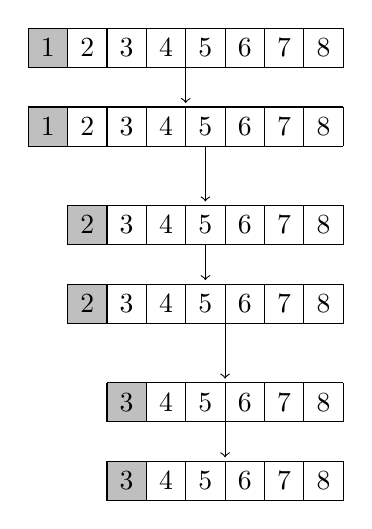
\begin{tikzpicture}[scale=0.5]
\begin{scope}
\fill[color=lightgray] (0,0) rectangle (1,1);
\draw (0,0) grid (8,1);
\foreach \x/\v in {0/1,1/2,2/3,3/4,4/5,5/6,6/7,7/8} \node at (0.5+\x,0.5) {\v};
\fill[color=lightgray] (0,-2) rectangle (1,-1);
\draw (0,-2) grid (8,-1);
\foreach \x/\v in {0/1,1/2,2/3,3/4,4/5,5/6,6/7,7/8} \node at (0.5+\x,-1.5) {\v};
\draw[->] (4,-0) -- (4,-0.9);
\draw[->] (4.5,-2) -- (4.5,-3.4);
\end{scope}
\begin{scope}[xshift=1cm,yshift=-4.5cm]
\fill[color=lightgray] (0,0) rectangle (1,1);
\draw (0,0) grid (7,1);
\foreach \x/\v in {0/2,1/3,2/4,3/5,4/6,5/7,6/8} \node at (0.5+\x,0.5) {\v};
\fill[color=lightgray] (0,-2) rectangle (1,-1);
\draw (0,-2) grid (7,-1);
\foreach \x/\v in {0/2,1/3,2/4,3/5,4/6,5/7,6/8} \node at (0.5+\x,-1.5) {\v};
\draw[->] (3.5,-0) -- (3.5,-0.9);
\draw[->] (4,-2) -- (4,-3.4);
\end{scope}
\begin{scope}[xshift=2cm,yshift=-9cm]
\fill[color=lightgray] (0,0) rectangle (1,1);
\draw (0,0) grid (6,1);
\foreach \x/\v in {0/3,1/4,2/5,3/6,4/7,5/8} \node at (0.5+\x,0.5) {\v};
\fill[color=lightgray] (0,-2) rectangle (1,-1);
\draw (0,-2) grid (6,-1);
\foreach \x/\v in {0/3,1/4,2/5,3/6,4/7,5/8} \node at (0.5+\x,-1.5) {\v};
\draw[->] (3,-0) -- (3,-0.9);
\end{scope}
\end{tikzpicture}
\caption{Pikajärjestämisen pahin tapaus: jokaisessa jaossa kaikki
alkiot jäävät jakoalkion toiselle puolelle.}
\label{fig:pikpah}
\end{figure}

Oma lukunsa on tilanne, jossa taulukossa on paljon samoja alkioita,
ääri\-tapauksena jokainen alkio on sama.
Tällöin tässä esitetty funktio \texttt{jako} tuottaa aina huonon jaon,
jossa kaikki alkiot menevät jakoalkion oikealle puolelle.
Ei siis riitä, että jakoalkio on valittu hyvin,
vaan myös tapa, jolla alkioita siirretään taulukossa,
vaikuttaa algoritmin tehokkuuteen.

Miten meidän tulisi sitten toteuttaa pikajärjestäminen?
Algoritmista on kehitetty vuosien aikana suuri määrä muunnelmia,
jotka pyrkivät parantamaan sen toimintaa eri tilanteissa.
Yksi kehittyneempi tapa valita jakoalkio on ottaa tarkasteluun
taulukon ensimmäinen, keskimmäinen ja viimeinen alkio ja valita
jakoalkioksi järjestyksessä keskimmäinen näistä kolmesta alkiosta.
Tällainen valinta toimii käytännössä hyvin monissa tilanteissa.
Parempi tapa toteuttaa alkioiden siirtäminen on puolestaan
käydä läpi rinnakkain alkioita alusta ja lopusta ja
pitää huoli siitä, että jakokohta jää keskelle, jos kaikki alkiot
ovat yhtä suuria.

\subsection{Algoritmien vertailua}

Meillä on nyt siis kaksi rekursiivista järjestämisalgoritmia:
lomitusjärjestä\-minen toimii \emph{aina} ajassa $O(n \log n)$,
kun taas pikajärjestäminen toimii \emph{ehkä} ajassa $O(n \log n)$,
mutta saattaa viedä aikaa $O(n^2)$.
Vaatii monenlaista virittelyä,
ennen kuin pikajärjestämisen saa toimimaan tehokkaasti
edes tapauksissa, joissa taulukko on valmiiksi järjestyksessä
tai kaikki alkiot ovat samoja.
Miksi haluaisimme koskaan käyttää epävarmaa pikajärjestämistä,
kun voimme käyttää myös varmasti tehokasta lomitusjärjestämistä?

\index{vakiokerroin}

Syynä on, että pikajärjestämisen \emph{vakiokertoimet} ovat pienet.
Kokemus on osoittanut, että kun toteutamme lomitusjärjestämisen ja
pikajärjestämisen ja mittaamme algoritmien todellisia suoritusaikoja,
pikajärjestäminen toimii usein nopeammin.
Näin tapahtuu siitä huolimatta, että pikajärjestämisen pahimman
tapauksen aikavaativuus on $O(n^2)$.
Käytännössä pahin tapaus on kuitenkin harvinainen,
jos jakoalkion valinta ja alkioiden siirtäminen on toteutettu huolellisesti.

\index{hybridialgoritmi}

Jos taulukko on pieni, $O(n^2)$-aikainen lisäysjärjestäminen
toimii käytän\-nössä nopeammin kuin rekursiiviset algoritmit,
koska sen vakiokertoimet ovat hyvin pienet.
Yksi mahdollisuus onkin toteuttaa \emph{hybridialgoritmi},
jossa suuret taulukot järjes\-tetään rekursiivisesti
ja pienet taulukot järjes\-tetään lisäysjärjestämisellä.
Tällöin eri algoritmien hyvät puolet pääsevät osaksi
kokonaisalgoritmia.
Käytännössä hybridialgoritmin voi tehdä niin,
että valitaan jokin sopiva raja $k$ ja
taulukko järjestetään rekursiivisesti,
jos siinä on ainakin $k$ alkiota, ja muuten lisäysjärjestämisellä.

\section{Järjestämisen alaraja}

Olisiko mahdollista luoda järjestämisalgoritmi, joka toimisi
nopeammin kuin $O(n \log n)$?
Osoittautuu, että tämä \emph{ei} ole mahdollista,
jos oletamme, että algoritmin tulee perustua taulukon
alkioiden vertailuihin.
Vertailuihin perustuva järjestämisalgoritmi järjestää taulukon
tekemällä joukon vertailuja muotoa
''onko alkio $x$ suurempi kuin alkio $y$?''.

Vertailuihin perustuva järjestämisalgoritmi on \emph{yleiskäyttöinen}:
se pystyy järjestämään mitä tahansa alkioita,
kunhan meillä on keino saada selville kahden alkion suuruusjärjestys.
Tämä on ominaisuus, jota yleensä ottaen toivomme
järjestämisalgoritmilta, joten vertailuihin perustuminen
on luonteva rajoitus.
Kaikki tähän mennessä käsittelemämme järjestämisalgoritmit
ovat olleet vertailuihin perustuvia

\subsection{Alarajatodistus}

Voimme ajatella vertailuihin perustuvaa järjestämistä
\emph{prosessina}, jossa jokainen vertailu antaa meille tietoa
taulukosta ja auttaa meitä viemään taulukkoa lähemmäs järjestystä.
Oletamme seuraavaksi, että taulukko muodostuu alkioista
$1,2,\dots,n$, jolloin meillä on $n!$ vaihtoehtoa, mikä
on taulukon alkuperäinen järjestys.
Jotta järjestämisalgoritmi voisi toimia oikein,
sen täytyy käsitellä jokainen järjestys eri tavalla.

Esimerkiksi jos $n=3$, taulukon mahdolliset järjestykset alussa ovat
$[1,2,3]$, $[1,3,2]$, $[2,1,3]$, $[2,3,1]$, $[3,1,2]$ ja $[3,2,1]$.
Algoritmi voi vertailla ensin vaikkapa ensimmäistä ja toista alkiota.
Jos ensimmäinen alkio on pienempi, voimme päätellä,
että mahdolliset taulukot ovat $[1,2,3]$, $[1,3,2]$ ja $[2,3,1]$.
Jos taas ensimmäinen alkio on suurempi,
mahdolliset taulukot ovat $[2,1,3]$, $[3,1,2]$ ja $[3,2,1]$.
Tämän jälkeen voimme jatkaa vertailuja samaan tapaan
ja saada lisää tietoa taulukosta.
Algoritmi voi päättyä vasta silloin, kun jäljellä on vain yksi
mahdollinen taulukko, jotta voimme olla varmoja, että olemme
järjestäneet taulukon oikein.

Tärkeä seikka on, että jokaisessa vertailussa ainakin puolet jäljellä
olevista taulukoista voi täsmätä vertailun tulokseen.
Niinpä jos algoritmilla käy huono tuuri, se voi enintään puolittaa
taulukoiden määrän joka askeleella.
Tämä tarkoittaa, että algoritmi joutuu tekemään pahimmassa
tapauksessa ainakin $\log(n!)$ vertailua.
Logaritmien laskusääntöjen perusteella
\[
\log(n!) = \log(1)+\log(2)+\dots+\log(n).
\]
Saamme tälle summalle alarajan ottamalla huomioon vain
$n/2$ viimeistä termiä ja arvioimalla niitä alaspäin niin, 
että jokaisen termin suuruus on vain $\log(n/2)$. Tuloksena on alaraja
\[
\log(n!) \ge (n/2) \log(n/2),
\]
mikä tarkoittaa, että algoritmi joutuu tekemään
pahimmassa tapauksessa $\Omega(n \log n)$ vertailua.

\subsection{Laskemisjärjestäminen}

\index{laskemisjärjestäminen}

Millainen olisi sitten järjestämisalgoritmi,
joka ei perustu vertailuihin ja toimii
tehokkaammin kuin $O(n \log n)$?
\emph{Laskemisjärjestäminen} on $O(n)$-aikainen järjestämisalgoritmi,
jonka toiminta perustuu oletukseen, että taulukon alkiot
ovat sopivan pieniä kokonaislukuja.
Tarkemmin ottaen algoritmi olettaa, että jokainen luku on
kokonaisluku välillä $0 \dots k$, missä $k=O(n)$.

Algoritmi luo \emph{kirjanpidon}, joka kertoo,
montako kertaa mikä\-kin mahdollinen luku välillä $0 \dots k$
esiintyy taulukossa.
Seuraavassa koodissa kirjanpito tallennetaan
taulukkoon \texttt{laskuri} niin, että
$\texttt{laskuri}[x]$ ilmaisee,
montako kertaa luku $x$ esiintyy taulukossa.
Tämän kirjanpidon avulla voimme luoda suoraan
lopullisen järjestetyn taulukon.

\begin{code}
for i = 0 to n-1
    laskuri[taulu[i]]++
i = 0
for x = 0 to k
    for j = 1 to laskuri[x]
        taulu[i] = x
        i++
\end{code}

Algoritmin molemmat vaiheet vievät aikaa $O(n)$,
joten se toimii ajassa $O(n)$ ja on käytännössä hyvin tehokas.
Algoritmi ei ole kuitenkaan yleinen järjestämisalgoritmi,
koska sitä voi käyttää vain silloin,
kun taulukon kaikki alkiot ovat sopivan pieniä kokonaislukuja.


\section{Järjestäminen Javassa}

Vaikka on hyödyllistä tuntea järjestämisen teoriaa,
käytännössä ei ole hyvä idea toteuttaa itse
järjestämisalgoritmia, koska nykypäivän ohjelmointikielissä
on valmiit työkalut järjestämiseen.
Valmiin algoritmin käyttämisessä on etuna,
että se on varmasti hyvin toteutettu ja tehokas.
Lisäksi meiltä säästyy aikaa, kun emme joudu
toteuttamaan algoritmia itse.

Javan standardikirjasto sisältää metodin \texttt{Arrays.sort},
joka järjestää sille annetun taulukon.
Esimerkiksi seuraava koodi järjestää kokonaislukuja
sisältävän taulukon:

\begin{code}
int[] taulu = {4,2,5,8,2,1,5,6};
Arrays.sort(taulu);
\end{code}

Kiinnostava kysymys on, mitä algoritmia Java käyttää
taulukon järjes\-tämiseen.
Asian voi tarkastaa Javan standardikirjaston
dokumentaatiosta.
Yllättävää kyllä, Javan käyttämä algoritmi riippuu siitä,
minkä \emph{tyyppistä} tietoa taulukossa on.
Jos taulukon alkiot ovat alkeistyyppisiä
(esimerkiksi \texttt{int}), Java käyttää 
pikajärjestämisen muunnelmaa,
jossa on kaksi jakoalkiota.
Jos taas alkiot ovat oliotyyppisiä
(esimerkiksi \texttt{String}),
algoritmina on optimoitu lomitusjärjestäminen.

Kun \texttt{Arrays.sort} järjestää olioita sisältävän taulukon,
se kutsuu metodia \texttt{compareTo} aina, kun se haluaa selvittää
kahden alkion suuruusjärjestyksen.
Metodin tulee palauttaa negatiivinen arvo, nolla tai positiivinen arvo
sen mukaan, onko olio itse pienempi, yhtä suuri vai suurempi
kuin parametrina annettu olio.
Javan omissa luokissa tällainen metodi on olemassa valmiina.
Esimerkiksi voimme tutkia merkkijonojen suuruusjärjestystä näin:

\begin{code}
System.out.println("apina".compareTo("banaani")); // -1
System.out.println("banaani".compareTo("apina")); // 1
System.out.println("apina".compareTo("apina")); // 0
\end{code}

Tämän ansiosta voimme järjestää suoraan taulukoita,
joissa on esimerkiksi merkkijonoja.
Jos haluamme, että Java pystyy järjestämään omia olioitamme,
meidän täytyy toteuttaa itse luokkaan metodi \texttt{compareTo} ja
merkitä, että luokka toteuttaa rajapinnan \texttt{Comparable}.
Esimerkiksi seuraava koodi toteuttaa luokan \texttt{Piste},
johon voidaan tallentaa pisteen x- ja y-koordinaatit.
Luokassa on metodi \texttt{compareTo}, joka määrittelee,
että pisteet järjestetään ensisijaisesti x-koordinaatin ja
toissijaisesti y-koordinaatin mukaan.

\begin{code}
public class Piste implements Comparable<Piste> {
    public int x, y;

    public int compareTo(Piste p) {
        if (this.x != p.x) {
            return this.x-p.x;
        } else {
            return this.y-p.y;
        }
    }
}
\end{code}

Metodin \texttt{compareTo} avulla voimme myös konkreettisesti
tarkastella, mitä Java tekee järjestäessään taulukon.
Seuraava luokka sisältää vain yhden luvun,
mutta ilmoittaa meille aina, kun Java kutsuu
\texttt{compareTo}-funktiota:

\begin{code}
public class Luku implements Comparable<Luku> {
    public int luku;

    public int compareTo(Luku x) {
        System.out.println("vertailu: " + luku + " " + x.luku);
        return this.luku-x.luku;
    }
}
\end{code}

Esimerkiksi kun järjestettävänä taulukkona on $[4,1,3,2]$,
saamme tietää, että Java tekee seuraavat vertailut:

\begin{code}
vertailu: 1 4
vertailu: 3 1
vertailu: 3 4
vertailu: 3 1
vertailu: 2 3
vertailu: 2 1
\end{code}

\section{Järjestämisen sovelluksia}

Järjestämisen merkitys algoritmiikassa on siinä,
että voimme ratkaista monia ongelmia tehokkaasti, 
kunhan aineisto on järjestyksessä.
Niinpä yleinen tapa luoda tehokas algoritmi on järjestää
ensin syöte ajassa $O(n \log n)$ ja hyödyntää sitten
tavalla tai toisella järjestystä algoritmin loppuosassa.

\subsection{Taulukkoalgoritmeja}

\label{sec:taukas}

Järjestämisen avulla voimme ratkaista ajassa
$O(n \log n)$ monia taulukoihin liittyviä tehtäviä.
Käymme seuraavaksi läpi kaksi tällaista tehtävää.

Ensimmäinen tehtävämme on laskea,
montako \emph{eri} alkiota annetussa taulukossa on.
Esimerkiksi taulukko $[2,1,4,2,4,2]$ sisältää kolme
eri alkiota: $1$, $2$ ja $4$.
Voimme ratkaista tehtävän järjestämällä ensin taulukon,
minkä jälkeen yhtä suuret alkiot ovat vierekkäin.
Tämän jälkeen tehtävän ratkaisu käy helposti,
koska riittää tutkia, monessako taulukon kohdassa on
\emph{vierekkäin} kaksi eri alkiota.
Voimme toteuttaa algoritmin näin:

\begin{code}
sort(taulu)
laskuri = 1
for i = 1 to n-1
    if taulu[i-1] != taulu[i]
        laskuri++
print(laskuri)
\end{code}

Algoritmi järjestää ensin taulukon ajassa $O(n \log n)$,
minkä jälkeen se käy läpi taulukon sisällön for-silmukalla
ajassa $O(n)$.
Tämän ansiosta algoritmi vie aikaa yhteensä $O(n \log n)$.


Entä jos haluammekin selvittää, mikä on taulukon \emph{yleisin} alkio?
Esimerkiksi taulukon $[2,1,4,2,4,2]$ yleisin alkio on $2$,
joka esiintyy kolme kertaa taulukossa.
Tämäkin tehtävä ratkeaa järjestämisen avulla, koska
järjestämisen jälkeen yhtä suuret alkiot ovat peräkkäin ja
meidän riittää etsiä pisin samaa alkiota toistava osuus.
Voimme toteuttaa algoritmin seuraavasti:

\begin{code}
sort(taulu)
maara = 1
suurin = 1
yleisin = taulu[0]
for i = 1 to n-1
    if taulu[i-1] != taulu[i]
        maara = 0
    maara++
    if maara > suurin
        suurin = maara
        yleisin = taulu[i]
print(yleisin)
\end{code}

Tässäkin algoritmissa järjestäminen vie aikaa $O(n \log n)$ ja
for-silmukka vie aikaa $O(n)$, joten algoritmin
kokonaisaikavaativuus on $O(n \log n)$.

\subsection{Binäärihaku}

\index{binäärihaku}

\emph{Binäärihaku} on menetelmä, jonka avulla voimme löytää alkion
järjestetystä taulukosta ajassa $O(\log n)$.
Ideana on pitää yllä hakuväliä, jossa etsittävä alkio voi olla,
ja puolittaa väli joka askeleella tutkimalla välin
keskimmäisenä olevaa alkiota.
Koska taulukko on järjestyksessä, voimme aina päätellä,
kumpaan suuntaan hakua tulee jatkaa.

Seuraava koodi etsii binäärihaulla taulukosta alkiota $x$:

\begin{code}
a = 0
b = n-1
while a <= b
    k = (a+b)/2
    if taulu[k] == x
        // alkio löytyi
        break
    if taulu[k] < x
        a = k+1
    if taulu[k] > x
        b = k-1
\end{code}

Algoritmi pitää yllä hakuväliä $[a,b]$, joka on aluksi $[0,n-1]$,
koska alkio $x$ saattaa olla missä tahansa kohdassa taulukossa.
Joka askeleella algoritmi tarkastaa välin keskellä kohdassa
$k=\lfloor (a+b)/2 \rfloor$ olevan alkion.
Jos kyseinen alkio on $x$, haku päättyy.
Jos taas alkio on pienempi kuin $x$, haku jatkuu välin
oikeaan puoliskoon,
ja jos alkio on suurempi kuin $x$, haku jatkuu välin
vasempaan puoliskoon.
Koska välin koko puolittuu joka askeleella,
binäärihaun aikavaativuus on $O(\log n)$.

\begin{figure}
\center
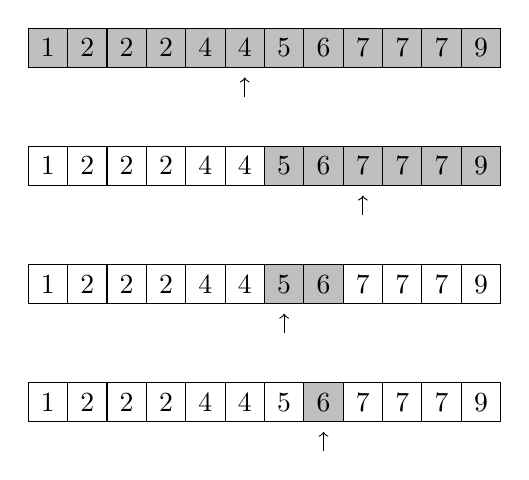
\begin{tikzpicture}[scale=0.5]
\begin{scope}
\fill[color=lightgray] (0,0) rectangle (12,1);
\draw (0,0) grid (12,1);
\foreach \x/\v in {0/1,1/2,2/2,3/2,4/4,5/4,6/5,7/6,8/7,9/7,10/7,11/9} \node at (0.5+\x,0.5) {\v};
\draw[->] (5.5,-0.75) -- (5.5,-0.25);
\end{scope}
\begin{scope}[yshift=-3cm]
\fill[color=lightgray] (6,0) rectangle (12,1);
\draw (0,0) grid (12,1);
\foreach \x/\v in {0/1,1/2,2/2,3/2,4/4,5/4,6/5,7/6,8/7,9/7,10/7,11/9} \node at (0.5+\x,0.5) {\v};
\draw[->] (8.5,-0.75) -- (8.5,-0.25);
\end{scope}
\begin{scope}[yshift=-6cm]
\fill[color=lightgray] (6,0) rectangle (8,1);
\draw (0,0) grid (12,1);
\foreach \x/\v in {0/1,1/2,2/2,3/2,4/4,5/4,6/5,7/6,8/7,9/7,10/7,11/9} \node at (0.5+\x,0.5) {\v};
\draw[->] (6.5,-0.75) -- (6.5,-0.25);
\end{scope}
\begin{scope}[yshift=-9cm]
\fill[color=lightgray] (7,0) rectangle (8,1);
\draw (0,0) grid (12,1);
\foreach \x/\v in {0/1,1/2,2/2,3/2,4/4,5/4,6/5,7/6,8/7,9/7,10/7,11/9} \node at (0.5+\x,0.5) {\v};
\draw[->] (7.5,-0.75) -- (7.5,-0.25);
\end{scope}
\end{tikzpicture}
\caption{Luvun 6 etsiminen järjestetystä taulukosta binäärihaun avulla.
Harmaa alue vastaa väliä $[a,b]$ ja nuoli osoittaa kohdan $k$.}
\label{fig:binhak}
\end{figure}

Kuva \ref{fig:binhak} näyttää esimerkin binäärihaun toiminnasta,
kun etsimme lukua 6 järjestetystä taulukosta.
Aluksi hakuvälinä on koko taulukko ja puolivälin kohdalla
on luku 4.
Niinpä voimme päätellä, että jos taulukossa on luku 6,
sen täytyy esiintyä taulukon loppuosassa.
Tämän jälkeen hakuvälinä on taulukon loppuosa ja
puolivälin kohdalla on luku 7.
Nyt voimme taas päätellä, että luvun 6 täytyy olla
tämän kohdan vasemmalla puolella.
Hakuväli puolittuu joka askeleella,
ja kun jatkamme vastaavasti, kahden askeleen kuluttua
hakuvälillä on vain yksi luku, joka on juuri haettu luku 6.
Olemme löytäneet halutun luvun ja algoritmi päättyy.

Voimme ratkaista binäärihaun avulla esimerkiksi tehtävän,
jossa annettuna on taulukko ja luku $x$ ja haluamme selvittää,
voimmeko valita taulukosta kaksi lukua $a$ ja $b$ niin, että $a+b=x$.
Järjestämme ensin taulukon, minkä jälkeen käymme läpi taulukon
luvut yksi kerrallaan.
Jokaisen luvun kohdalla tutkimme, voisiko kyseinen luku olla $a$.
Tällöin taulukossa pitäisi olla toinen luku $b$ niin, että
$a+b=x$, eli taulukossa pitäisi olla luku $x-a$.
Pystymme tarkastamaan tämän binäärihaulla ajassa $O(\log n)$.
Tuloksena on algoritmi, joka vie aikaa $O(n \log n)$,
koska sekä järjestäminen että binäärihakua käyttävä läpikäynti
vievät aikaa $O(n \log n)$.
